\documentclass[11pt, oneside]{article}   	% use "amsart" instead of "article" for AMSLaTeX format
\usepackage{geometry}                		% See geometry.pdf to learn the layout options. There are lots.
\geometry{letterpaper}                   		% ... or a4paper or a5paper or ... 
%\geometry{landscape}                		% Activate for for rotated page geometry
%\usepackage[parfill]{parskip}    		% Activate to begin paragraphs with an empty line rather than an indent
\usepackage{graphicx}				% Use pdf, png, jpg, or eps� with pdflatex; use eps in DVI mode
								% TeX will automatically convert eps --> pdf in pdflatex		
\usepackage{amssymb}
\usepackage{amsmath}
\usepackage{parskip}
\usepackage{color}

\title{Divergence}
%\author{The Author}
%\section{}
% \subsection*{R code}
\date{}							% Activate to display a given date or no date

\graphicspath{{/Users/telliott_admin/Dropbox/Tex/png/}}

% \begin{center} 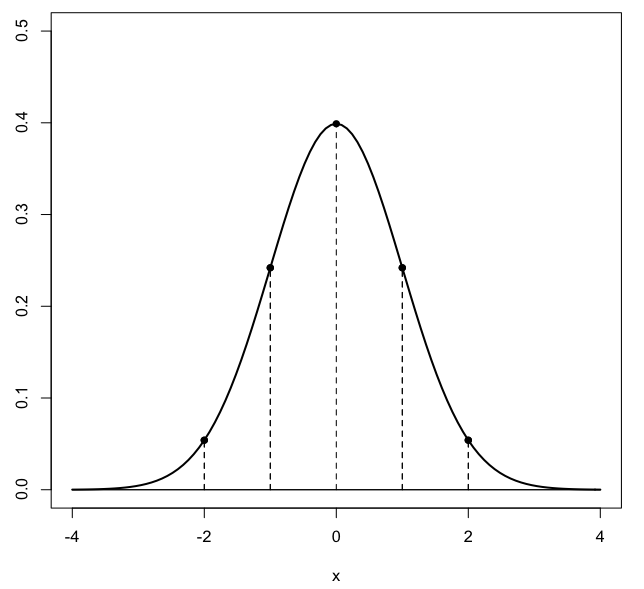
\includegraphics [scale=0.4] {gauss3.png} \end{center}
% \begin{bmatrix} a  &  b \\ c  &  d \end{bmatrix}
% \bigg |_

\begin{document}
\maketitle
\large
%\noindent

Green's Theorem is
\[ \oint_C \mathbf{F} \cdot \mathbf{dr} = \iint\limits_{R}  curl(\mathbf{F}) \ dA \]
\[ \oint_C M \ dx + N \ dy  = \iint\limits_{R} (N_x - M_y) \ dA \]
It can be used for finding area by computing a line integral.  The trick is to imagine an $M$ and $N$ such that
\[ N_x - M_y = 1 \]
because then we have
\[ \oint_C M \ dx + N \ dy  = \iint\limits_{R}  \ dA = Area \]
An especially common choice is:
\[ M = -\frac{y}{2}, \ \ N = \frac{x}{2} \]
So we have that
\[ A = \frac{1}{2} \oint_C x \ dy - y \ dx \]

Let's try this out on a circle.  What is the parametrization of $C$?  We need $x$ and $y$ as functions of $t$:
\[ x = a \ cos \ t \]
\[ dx = -a \ sin \ t  \ dt \]
\[ y = a \ sin \ t \]
\[ dy = a \ cos \ t  \ dt \]
\[ A = \frac{1}{2} \int_{t=0}^{t=2\pi} a^2 cos^2t \ dt + a^2 sin^2t \ dt \]
\[ = \frac{1}{2} \ a^2 \ 2 \pi = \pi a^2 \]

What about an ellipse?  What is the parametrization of $C$?  We need $x$ and $y$ as functions of $t$:
\[ x = a \ cos \ t, \]
\[ dx = -a \ sin \ t  \ dt \]
\[ y = b \ sin \ t \]
\[ dy = b \ cos \ t  \ dt \]
To see that the above is correct, do this
\[ \frac{x^2}{a^2} + \frac{y^2}{b^2} = cos^2 \ t + sin^2 \ t = 1 \]
Clearly the formula of an ellipse.  Now plug into the integral

\[ A = \frac{1}{2} \int_{t=0}^{t=2\pi} ab \ cos^2t \ dt + ab \ sin^2t \ dt \]
\[  \frac{1}{2} \ ab \ 2 \pi = \pi ab \]
Finally, what seems a very simple example:
the part of the rectangle $[0,1] \times [0,2]$ below the line $y=2x$,
is actually complicated because there are three segments of the curve:
\[ y = 2x \]
\[ dy = 2 \ dx \]
\[ A = \frac{1}{2} \oint_C x \ dy - y \ dx  \]
\[ C1:  x = 0 \to 1,\  y = 0 \]
\[ C2:  x = 1,\  y = 0 \to 2 \]
\[ C3:  y = 2x,\  x = 1 \to 0 \]
\[ M = -\frac{y}{2}, \ \ N = \frac{x}{2} \]
\[ A_1 = \frac{1}{2} \oint_C x \ dy - y \ dx = \frac{1}{2} \oint_C x \ 0 - 0 \ dx = 0  \]
\[ A_2 = \frac{1}{2} \oint_C x \ dy - y \ dx = \frac{1}{2} \oint_C 1 \ dy - y \ 0 = y \bigg |_0^2 = 1  \]
\[ A_3 = \frac{1}{2} \oint_C x \ dy - y \ dx = \frac{1}{2} \oint_C x \ 2 \ dx - 2x \ dx = 0  \]
The total area is just 1.

\subsection*{divergence example}
Verify the divergence theorem for a hemisphere of radius $a$ with $\mathbf{F} = \langle x,y,z \rangle$.
Restate the theorem
\[ \iint_S \ \mathbf{F} \cdot \hat{\mathbf{n}} \ dS = \iiint_D \ \nabla \cdot \mathbf{F} \]

Noting that the field is given in $x,y,z$-coordinates, recall that
\[ \hat{\mathbf{n}} \ dS = a^2 \ \langle x,y,z \rangle   \ \sin \phi \ d \phi \ d \theta \]
So on the left side
\[ \mathbf{F} \cdot \hat{\mathbf{n}} \ dS = \langle x,y,z \rangle \cdot a^2 \langle x,y,z \rangle = a^3  \]
and
\[ = \iint_S a^3  \ \sin \phi \ d \phi \ d \theta \]
\[ = \int_S a^3  \ [ \ - \cos \phi \ \bigg |_0^{\pi/2}  \ ] \ d \theta \]
\[ = \int_S a^3  \ d \theta  = 2 \pi a^3 \]

Don't forget the bottom surface.  In this problem, there is a component of the field in the $z$ direction

\[ \mathbf{F} \cdot \hat{\mathbf{n}} \ dS =  \langle x,y,z \rangle \cdot  \langle 0,0,-1 \rangle \ dx \ dy = -z \ dx \ dy\]
however, the value of this field on the $xy$-plane is $z=0$ so there is no flux.


For the divergence,

\[ \nabla \cdot \mathbf{F} = 1 + 1 + 1 = 3 \]
which is pretty easy!.  Now, integrate
\[ \iiint_D \ 3 \ dV \]
Well, the volume is $\frac{2}{3} \pi a^3$ so we obtain $2 \pi a^3$.

\subsection*{OSU example}

A problem from OSU asks us to verify the divergence theorem for 
\[ \mathbf{F} = \ \langle y,x,z \rangle \]

where the region is
\[ 0 \le z \le 16 -x^2 -y^2 \]

The graph of $z=16 -x^2 -y^2$ is a paraboloid which opens downward and has its vertex at $z=16$.  When $z=0$ we have a circle of radius $r=4$.

Recall that 
\[ \hat{\mathbf{n}} \ dS = \langle -f_x,-f_y,1 \rangle  \ dA \]
 so for this paraboloid surface we have
 \[ z = f(x,y) = 16 - x^2 - y^2 \]
\[ \hat{\mathbf{n}} \ dS = \ \langle 2x,2y,1 \rangle  \ dA \]
This corresponds to $\hat{\mathbf{n}}$ pointing out of the surface.
Then
\[ \iint_S \mathbf{F} \cdot \hat{\mathbf{n}} \ dS  = \iint_R 4xy + z \ dA \]
\[ =  \int_{-4}^{4} \int_{-\sqrt{16-y^2}}^{\sqrt{16-y^2}} \ 4xy + 16 - x^2 - y^2 \ dx \ dy \]

$xy$-coordinates are not a good way to do this problem.  Convert to polar coordinates
\[ x = r \cos \theta \]
\[ y = r \sin \theta \]
\[ dA = r \ dr \ d\theta \]
\[  \iint_R (4r^2 \sin \theta \cos \theta + 16 - r^2) \ r \ dr \ d\theta \]
The region of integration is the disk of radius $r=4$
\[ \int_0^{2\pi} \ \int_0^4 \ (4 r^2 \sin \theta \cos \theta + 16 - r^2) \ r \ dr \ d \theta \]
The inner integral is
\[ \int_0^4 \ 4 r^3 \sin \theta \cos \theta + 16r - r^3 \ dr \]
\[ r^4  \sin \theta \cos \theta + 8r^2 - \frac{1}{4}r^4 \ \bigg |_0^4 \]
\[ = 256   \sin \theta \cos \theta + 128 - 64 \]
\[ = 256   \sin \theta \cos \theta + 64 \]
The outer integral is
\[ \int_0^{2\pi} 64 +  256  \sin \theta \cos \theta \ d \theta \]
\[ = 128 \pi + 256 \sin^2 \theta \bigg |_0^{2\pi} \]
\[ = 128 \pi  \]
There is another part of our solid.  That is the disk in the $xy$-plane.  For this disk, the unit normal (pointing out) is just $\langle 0,0,-1 \rangle$.
\[ \iint_S \mathbf{F} \cdot \hat{\mathbf{n}} \ dS  = -\iint_R z \ dA \]
but remember that we're on the $xy$-plane so $z=0$ and the whole integral is $0$.

We're not done yet!  We still have to compute
\[ \iiint_R \ \nabla \cdot \mathbf{F} \]
\[ = \iiint_R P_x + Q_y + R_z \ dV \]
since $\mathbf{F} = \ \langle y,x,z \rangle$ this is just equal to $3$.  So we need 
\[ 3 \iiint_R  \ dV \]
If we convert to cylindrical coordinates, we will integrate over the disk of radius $r=4$.  What is the upper bound on $z$?
\[ z = 16 - x^2 - y^2 = 16 - r^2 \]
So we have
\[ \int_0^{2\pi} \ \int_0^4 \ \int_0^{16 - r^2} \ dz \ r \ dr \ d \theta \]

The inner integral is just $16 - r^2$.  The middle integral is
\[ \int_0^4 16r - r^3 \ dr \]
\[ = 8r^2 - \frac{1}{4}r^4 \ \bigg |_0^4 \]
\[ = 128 - 64 = 64 \]
Finally, we pick up $2 \pi$ from the outer integral for a final result of $128 \pi$, which matches what we had above.

Or, we could have just said that the solid is a hemisphere of radius $4$ so the volume is a standard formula.  Again, we need 
\[ 3 \iiint_R  \ dV \]
so
\[ 3 V = 3 \ \frac{1}{2} \ \frac{4}{3} \pi 4^3 \]
$16^2 = 256$ and one-half of that is $128$, times $\pi$.


\end{document}  